%This is my super simple Real Analysis Homework template

\documentclass{article}
% \usepackage[utf8]{inputenc}
\usepackage[english]{babel}
\usepackage[]{amsthm} %lets us use \begin{proof}
\usepackage[]{amssymb} %gives us the character \varnothing
\usepackage{geometry}
\usepackage{graphicx}
\graphicspath{ {} }
\geometry{legalpaper, margin=1.2in}
% \usepackage{xeCJK}
% \setCJKmainfont{cwTeXFangSong}
\title{Homework 1}
\author{Chun-Hui,Wu}
\date\today
%This information doesn't actually show up on your document unless you use the maketitle command below

\begin{document}
\maketitle %This command prints the title based on information entered above



\subsection*{Problem 1}
Proof Convexity inequality by induction.
\begin{proof}
If $f$is convex on closed interval $\left[ a,b\right]$, then given $\lambda \in \left[ 0,1\right]$ ,$f$ satisfies $$f(\lambda a+(1-\lambda b))\leq \lambda f(a) + (1-\lambda)f(b)$$
We now prove , given $\lambda_{1},\lambda_{2}...\lambda_{n} $ satisfies $\sum_{i=1}^{M}\lambda_{i}=1 , \lambda \geq 0$ , $f$ satisfies \\[5pt] $$f(\sum_{i=1}^{M}\lambda_{i}x_{i}) \leq \sum_{i=1}^{M}\lambda_{i}f(x_{i})\\$$\\[5pt]
The inequality hold for $M=1,2$.Suppose the inequality holds for $M=n$.
We now check if the inequality hold for $M=n+1$

\begin{eqnarray}
   f(\sum_{i=1}^{n+1}\lambda_{i}x_{i})&=& f(\sum_{i=1}^{n}\lambda_{i}x_{i}+\lambda_{n+1}x_{n+1})\\
   	                                  &=& f((1-\lambda_{n+1})\sum_{i=1}^{n}\frac{\lambda_{i}}{1-\lambda_{n+1}}x_{i}+\lambda_{n+1}x_{n+1})\\
                                      &\leq& (1-\lambda_{n+1}) f(\sum_{i=1}^{n}\frac{\lambda_{i}}{1-\lambda_{n+1}}x_{i})+\lambda_{n+1}f(x_{n+1})\\ 
                                      &\leq& (1-\lambda_{n+1}) \sum_{i=1}^{n}\frac{\lambda_{i}}{1-\lambda_{n}}f(x_{i})+\lambda_{n+1}f(x_{n+1})\\
                                      &=& \sum_{i=1}^{n}\lambda_{i}f(x_{i})+\lambda_{n+1}f(x_{n+1})\\
                                      &=& \sum_{i=1}^{n+1}\lambda_{i}f(x_{i})
\end{eqnarray}

In (3) we use the fact that $\sum_{i=1}^{n}\frac{\lambda_{i}}{1-\lambda_{n+1}}=1$ since the inequality holds.\\
In (4) we use the assumpsion of "M=n" , since the inequality holds.
Finally , we prove the convexity inequality by induction.

\end{proof}

\clearpage %Gives us a page break before the next section. Optional.
\subsection*{Problem 2}
Derive the entropy of the univariate Gaussian.
\begin{proof}
Given Random variable  $X$ , the entropy is defined by $$H[X]:=E[I[X]]=E[-ln(X)]$$
We now consider univariate Gaussian random variable and derive its entropy.
By the definition of entropy $$H[X]=E[-ln(X)] = -\int_{\Omega}p(x)ln(p(x))dx$$
since X is a Gaussian Random Variable,
\begin{eqnarray}
  H[X] &=& -\int_{-\infty}^{\infty}\frac{1}{\sqrt[]{2\pi}\sigma}e^\frac{-(x-\mu)^2}{2\sigma^2}ln(\frac{1}{\sqrt[]{2\pi}\sigma}e^\frac{(x-\mu)^2}{2\sigma^2})dx\\[5pt]
          &=& -\int_{-\infty}^{\infty}\frac{1}{\sqrt[]{2\pi}\sigma}e^\frac{-(x-\mu)^2}{2\sigma^2}(ln(\frac{1}{\sqrt[]{2\pi}\sigma})-\frac{(x-\mu)^2}{2\sigma^2})dx \\[5pt]
          &=& \frac{1}{2}ln(2\pi\sigma^2)+\int_{-\infty}^{\infty}\frac{1}{\sqrt[]{2\pi}\sigma}e^\frac{(x-\mu)^2}{2\sigma^2}\frac{(x-\mu)^2}{2\sigma^2}dx \\[5pt]
          &=&\frac{1}{2}ln(2\pi\sigma^2)+\int_{-\infty}^{\infty}\frac{1}{\sqrt[]{2\pi}}e^\frac{-a^2}{2}\frac{a^2}{2}da \\[5pt]
          &=&\frac{1}{2}ln(2\pi\sigma^2)+\frac{1}{2}
\end{eqnarray}\\[5pt]
From (9) to (10) we simply let $a=\frac{x-\mu}{\sigma}$,and apply the technics of change of variable.
From (10) to (11) we use the fact that $E[X^2]=\sigma^2+\mu^2 .$
\end{proof}

\subsection*{Problem 3}
Evaluate the KL divergence between two Gaussian.$p(x) = N(x|\mu,\sigma^2)$ and $q(x) = N(x|m,s^2)$.
\begin{proof}
K-L divergence is defined by $$KL(p||q):= -\int p(x)ln\frac{q(x)}{p(x)}dx = -\int p(x)ln(q(x))dx+\int p(x)ln(p(x))dx$$
Given $p(x) = N(x|\mu,\sigma^2)$ and $q(x) = N(x|m,s^2)$ , we derive the K-L divergence of p and q.
\begin{eqnarray}
  KL(p || q) &=& -\int p(x)ln(q(x))dx+\int p(x)ln(p(x))dx \\[5pt]
          &=& -\int p(x)ln(q(x))dx- \frac{1}{2}ln(2\pi\sigma^2)-\frac{1}{2}
\end{eqnarray}\\[5pt]
We calculate $\int p(x)ln(q(x))dx $  below.
\begin{eqnarray}
 \int p(x)ln(q(x))dx &=& \int \frac{1}{\sqrt[]{2\pi}\sigma}e^\frac{-(x-\mu)^2}{2\sigma^2} (ln(\frac{1}{\sqrt[]{2\pi}s})-\frac{(x-m)^2}{2s^2})dx \\[5pt]
          &=& ln(\frac{1}{\sqrt[]{2\pi}s})-\int_{-\infty}^{\infty}\frac{1}{\sqrt[]{2\pi}}e^\frac{-a^2}{2}\frac{(a\sigma+\mu-m)^2}{2s^2}da \\[5pt]
          &=&ln(\frac{1}{\sqrt[]{2\pi}s}) - \frac{1}{2s^2} \int (\sigma^2a^2+2\sigma(\mu-m)a+(\mu-m)^2)\frac{1}{\sqrt[]{2\pi}}e^\frac{-a^2}{2}da \\[5pt]
          &=& -\frac{1}{2}ln(2\pi s^2)- \frac{1}{2s^2}(\sigma^2+(\mu-m)^2)
\end{eqnarray}\\[5pt]
In (13) ,we use the result calculated in problem2.\\
In (15) ,we simply let $a=\frac{x-\mu}{\sigma}$,and apply the technics of change of variable.\\
Combine the result we just derive ,we know that 
\begin{eqnarray}
KL(p || q) &=& -\int p(x)ln(q(x))dx+\int p(x)ln(p(x))dx \\[5pt]
		   &=& -(-\frac{1}{2}ln(2\pi s^2)- \frac{1}{2s^2}(\sigma^2+(\mu-m)^2))- \frac{1}{2}ln(2\pi\sigma^2)-\frac{1}{2}\\[5pt]
           &=& ln(\frac{s}{\sigma})+\frac{1}{2s^2}(\sigma^2+(\mu-m)^2)-\frac{1}{2}
\end{eqnarray}\\[5pt]
\end{proof}

\subsection*{Problem 4}
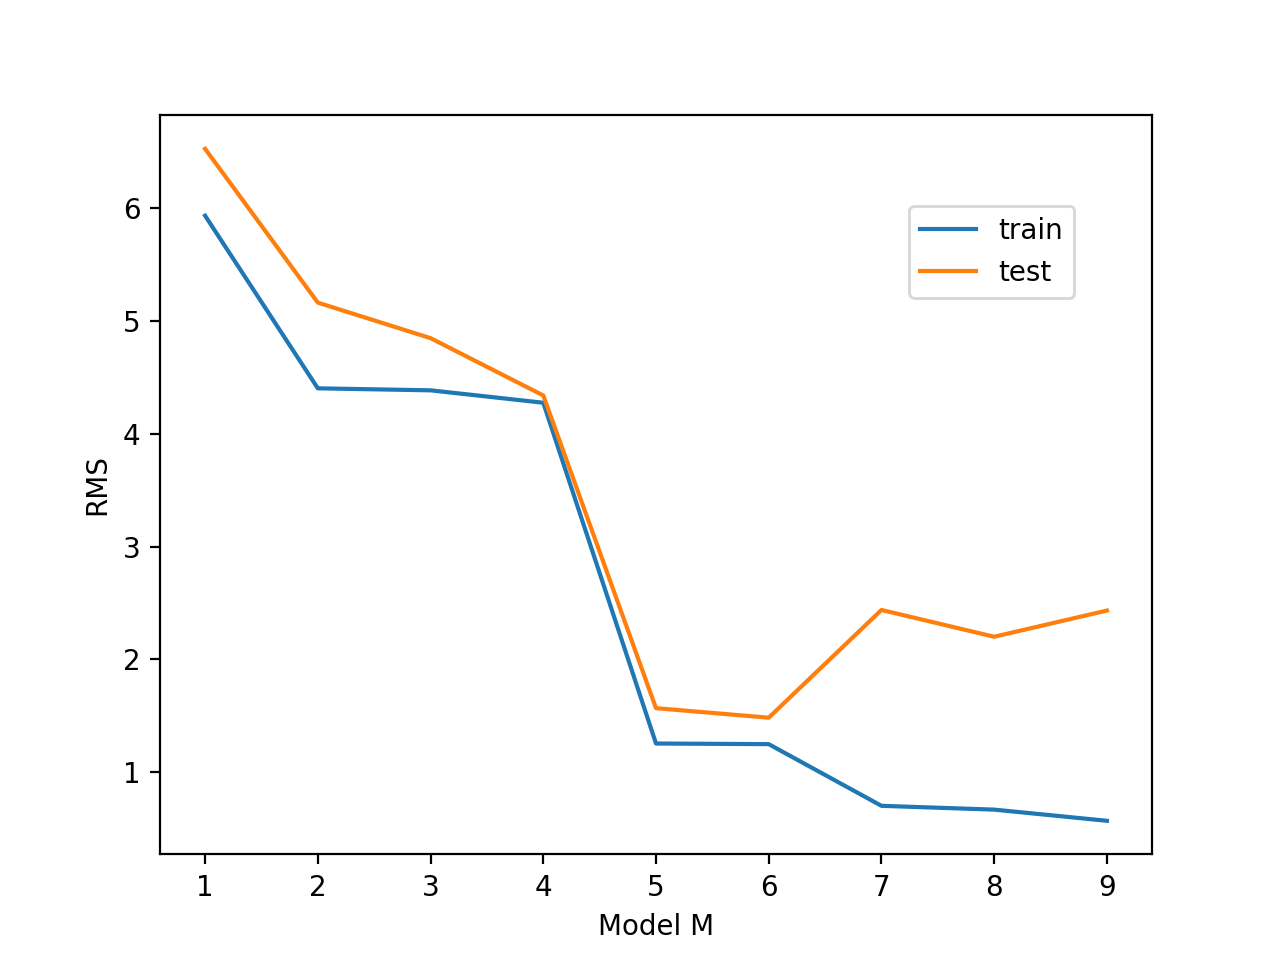
\includegraphics[width=\textwidth]{Figure_1.png}\\
When the order $M > 6 $, overfitting occurs.\\
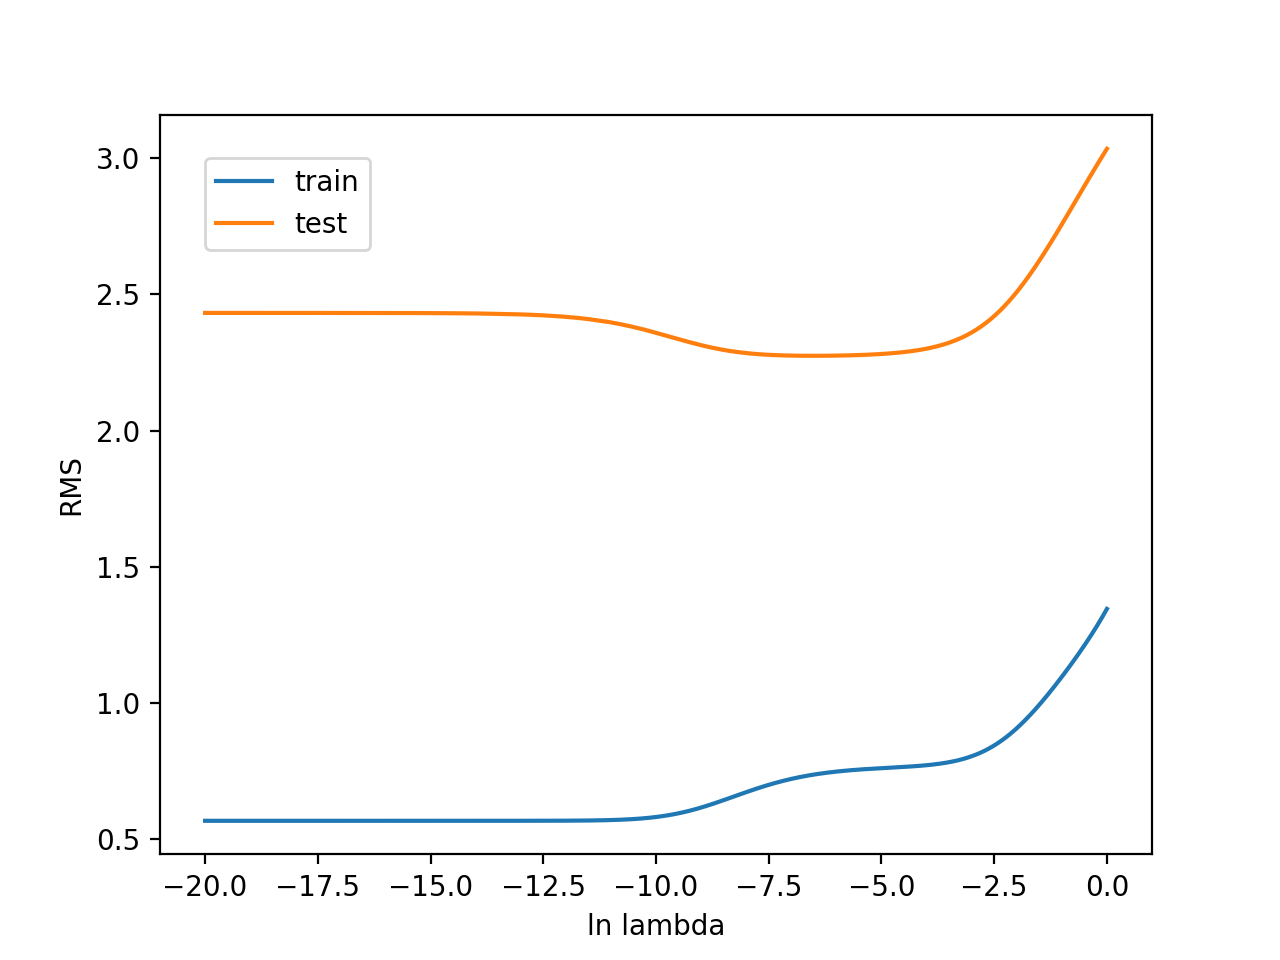
\includegraphics[width=\textwidth]{Figure_2.png}\\
I choose 1000 $ln(\lambda_i)$ uniformly  in $\left[-20,0\right]$ .

\subsection*{Problem 5}
\subsubsection*{1}
For $M = 1$,the training  $ RMS = 0.0512$ , the testing $RMS =0.0292$\\
For $M = 2$,the training  $ RMS = 0.0355$ , the testing $RMS =0.0349$\\
\subsubsection*{2}
Leave petal width out the training, the training  $ RMS = 0.0577$ , the testing $RMS = 0.0596$\\
Leave sepal width out the training, the training  $ RMS = 0.0554$ , the testing $RMS = 0.0263$\\
Leave petal length out the training, the training  $ RMS =0.0467 $ , the testing $RMS =0.0269$\\
Leave sepal length out the training, the training  $ RMS =0.0434 $ , the testing $RMS =0.0305$\\
So if the petal width is left ,the training $RMS$ would mostly increase  among the four attributes.So petal width is the most contributive attribute.



\end{document}